\section{How the Records Lose Data}
\label{sec:outages}

\subsection{Water-quality deployments: most missing data are in long gaps}
\label{sec:out-water}
Fig.~\ref{fig:records} shows when each record was down. Two features are visible at once: many short gaps, and a few gaps lasting days.

\begin{figure*}[t]
\centering
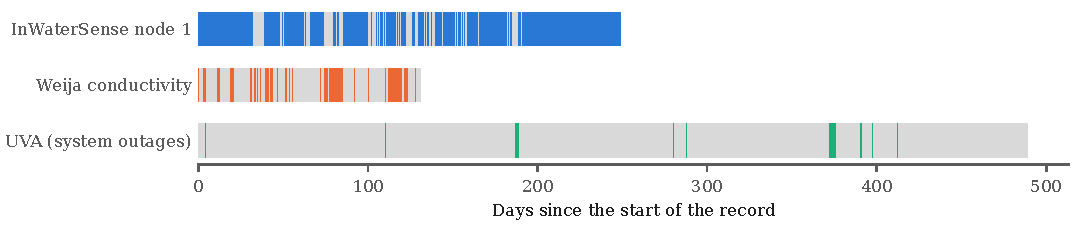
\includegraphics[width=\textwidth]{fig_records}
\caption{Delivery timelines of the three records with long gaps: coloured spans are slots in which nothing was delivered (UVA: system outages only; its short radio losses are not shown). Each record is drawn on its own time axis, from its first slot.}
\label{fig:records}
\end{figure*}

InWaterSense node~1 had \inwsOutages{} delivery gaps. Many were short: \inwsOneSlotEvents{} lasted a single slot, but together they held only \inwsOneSlotLost{} of the missing readings. At the other end, \inwsDayEvents{} gaps of a day or more (\inwsDayEventShare{} of all gaps) held \inwsDayLost{} of the missing readings (bootstrap 95\% CI \inwsDayLostLo--\inwsDayLostHi), and gaps of 6~h or more held \inwsSixLost{} (\inwsSixLostLo--\inwsSixLostHi). The longest lasted \inwsMaxOutageDays~days. Fig.~\ref{fig:outage-share} shows the whole curve.

The Weija deployment, on a different continent, shows the same structure. Its conductivity stream had \weijaCondOutages{} gaps and lost \weijaCondLoss{} of its readings; \weijaCondDayLost{} of the missing readings fell in gaps of a day or more, and the share was between \weijaDayLostMin{} and \weijaDayLostMax{} across all \weijaStreams{} streams, the longest gap lasting \weijaMaxOutageDays~days. With only \weijaCondDayN{} day-long gaps in the conductivity stream, its confidence interval is wide (\weijaCondDayLostLo--\weijaCondDayLostHi), so Weija is treated as qualitative support for the InWaterSense result rather than as a second estimate of it. As Sec.~\ref{sec:data-cause} showed, Weija's long gaps are silences of the whole node, and most of InWaterSense's long gaps were shared with the second node behind the same gateway.

\begin{figure}[t]
\centering
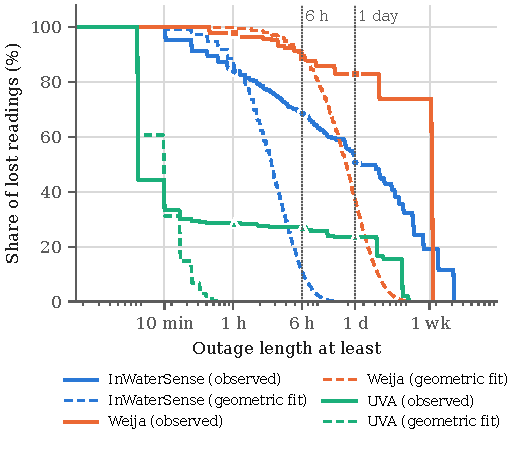
\includegraphics[width=\columnwidth]{fig_outage_share}
\caption{Share of missing readings that fall in gaps at least as long as the value on the horizontal axis, $S(L)$ in (\ref{eq:share}) (solid), and the same share predicted by the geometric model (\ref{eq:geo}) fitted to each record's gap lengths (dashed). Markers at 1~h, 6~h and 1~day. InWaterSense node~1 (611-s slots), Weija conductivity (\weijaCondStepMin-min slots) and UVA (all sensors, 5-min slots; radio and system losses together).}
\label{fig:outage-share}
\end{figure}

\subsection{The geometric gap-length model fails, and no tested model fits}
\label{sec:out-models}
Table~\ref{tab:aic} compares the four gap-length models (\ref{eq:geo})--(\ref{eq:pl}). The geometric model (\ref{eq:geo}), whose single loss state underlies both independent losses and the Gilbert--Elliott channel, ranks last on every record, by \aicGeomGapInws{} AIC points on InWaterSense, \aicGeomGapWeija{} on Weija and \aicGeomGapUva{} on UVA. Its failure is in exactly the quantity that matters, the long-gap share (\ref{eq:share}): fitted to InWaterSense, it puts \geomSixInws{} of the missing readings in gaps of 6~h or more, against \inwsSixLost{} observed, and \geomDayInws{} in gaps of a day or more, against \inwsDayLost{} (Fig.~\ref{fig:outage-share}). On Weija it puts \geomDayWeija{} in day-long gaps, against \weijaCondDayLost{}.
AIC only ranks the models, so each was also tested absolutely, by the bootstrap Kolmogorov--Smirnov test of Sec.~\ref{sec:data-outages}. The geometric model is rejected on every record ($p\le$\,\gofPmin, the smallest value the 200 bootstrap samples can give). With \gofInwsN{} gaps on InWaterSense and \gofUvaN{} runs on UVA, every tested model is rejected, but by very different margins: the geometric model's largest distance between fitted and observed distribution functions is \gofGeomDInws{} on InWaterSense and \gofGeomDUva{} on UVA, against \gofBestDInws{} and \gofBestDUva{} for the best of the other models. On Weija's few gaps, the lognormal and power-law models are not rejected ($p=$\,\gofWeijaLnP{} and \gofWeijaPlP). The ranking is not driven by one extreme gap: without the longest gap of each record, every record keeps its best model. A geometric gap-length model is thus strongly unsupported relative to the alternatives tested, and no tested model describes the larger records exactly.

No single alternative wins everywhere. The discrete lognormal is best by AIC on InWaterSense, the discrete power law on Weija (with the lognormal \aicWeijaLnGap{} AIC points behind), and the two-geometric mixture on UVA. The mixture's form, many short losses and a few long gaps, is the common thread, and the records differ visibly in how many long gaps they have (Fig.~\ref{fig:outage-share}). Gaps are also not independent of each other. On InWaterSense a long gap tends to be followed by another long gap (Spearman $\rho=$\,\inwsRhoNextOut) and by a short up-run ($\rho=$\,\inwsRhoNextUp; both \inwsRhoP), so gaps cluster into bad periods that a renewal model, drawing each gap independently, cannot reproduce. On Weija, with \weijaCondOutages{} gaps, neither correlation is distinguishable from zero ($\rho=$\,\weijaRhoNextOut, $p=$\,\weijaPNextOut; $\rho=$\,\weijaRhoNextUp, $p=$\,\weijaPNextUp). For these reasons all simulations in this paper replay the real records rather than a fitted model.

\begin{table}[t]
\centering
\caption{AIC of gap-length models (lower is better; best per record in bold). UVA: all missing-frame runs of all sensors, 5-min slots.}
\label{tab:aic}
\small
\begin{tabular}{@{}lrrr@{}}
\toprule
Model & InWaterSense & Weija & UVA \\
\midrule
\tabin{tables/tab_outage_models.tex}
\bottomrule
\end{tabular}
\end{table}

\subsection{LoRaWAN networks: short radio losses and rare system outages}
\label{sec:out-lorawan}
The two LoRaWAN records separate the causes of loss. On LoED, well-heard devices lost \loedRadioLoss{} of their frames to the radio. Losses were mildly bursty: the probability of losing a frame after a lost frame was \loedCondLoss, about \loedCondRatio{} times the marginal rate. But the bursts were short: of \loedBursts{} radio-loss bursts, \loedBurstOne{} were a single frame and \loedBurstFive{} at most five frames. Losses also did not coincide across devices beyond what their density implies: a lost frame coincided with a loss of another device at a shared gateway within the same minute in \loedCoLoss{} of cases, against \loedCoLossBase{} (\loedCoLossLo--\loedCoLossHi) under a random time-shift baseline.

UVA adds what LoED, recorded in campaign windows, cannot show: 16 months of continuous operation. The system as a whole was available \uvaAvail{} of the time, with \uvaSysOutages{} system outages (median \uvaSysMedianH~h, longest \uvaSysMaxH~h). Of the \uvaMissing{} missing frames, \uvaRadioShare{} were radio losses and \uvaSysShare{} system losses. The radio regime looks like LoED's: \uvaRunsOne{} of the \uvaRuns{} runs of missing frames were a single frame. The system regime looks like the water-quality deployments': \uvaSysDayShare{} of the system down-time fell in outages of a day or more. With few system outages, UVA's long outages hold a smaller share of its missing frames than at InWaterSense (\uvaSixLost{} in runs of 6~h or more, \uvaDayLost{} in runs of a day or more; Fig.~\ref{fig:outage-share}). The classification is not an artefact of the 10-minute bin: with bins of 5 to 30~min the number of system outages ranges from \uvaBinOutMax{} to \uvaBinOutMin{} (short ones merge), the share of system down-time in outages of a day or more from \uvaBinDayMin{} to \uvaBinDayMax{}, and the system share of missing frames from \uvaBinSysMin{} to \uvaBinSysMax{}.

Two further observations matter for design. First, \emph{gateway diversity masks gateway outages}: one of UVA's gateways was down for \uvaGwCDays{} days in a row, yet none of the missing frames was a gateway loss, because every sensor was also heard by a second gateway. Second, rain had no detectable effect on link loss: over \uvaRainPairs{} sensor--gateway pairs, loss was \uvaRainDry{} in dry hours and \uvaRainWet{} in rainy hours (Wilcoxon signed-rank test~\cite{wilcoxon1945individual}, $p=$\,\uvaRainP).

In answer to RQ1: across the four records studied, losses separate into short radio losses, which are nearly independent, and rarer long delivery gaps or system outages of a gateway, its backhaul, the server or the node. In the two water-quality deployments, gaps of 6~h or more hold most of the missing data (\inwsSixLost{} on InWaterSense, \weijaCondSixLost{} on Weija conductivity). A geometric gap-length model misses the second regime almost entirely.
